\subsection{Standard Model Single Top}
\label{sec:Bkg:SingleTop}

\indent Standard Model single top consists of 3 to 7 percent of the background in any one $\RISR$ bin. In total, single top consist of 4 percent of the total background in SRC.  A 1 lepton single top control region is defined in section \ref{sec:SingleTopCR}.  The single top CR is orthogonal to both the 1 lepton $W$+jets control region and ttbar control region.  \\

\subsubsection{Single Top Control Region}
\label{sec:SingleTopCR}

\indent The definition of the single top control region is given in table \ref{tab:1CR_BaseDefs}. \\

\begin{table}[htpb]
  \caption{Selection for the 1-lepton, single top control region.}
  \begin{center}
    \begin{tabular}{c|c}
      \hline \hline
 	& CRST           \\ \hline
      Number of leptons             & 1                                            \\ 
      Number of jets (incl. lepton) & $\geq 4$                                     \\ 
      $\pt$ of jets (incl. lepton)  & (80,80,40,40) GeV                            \\ 
      \mindphijettwomet             & $> 0.4$                                      \\ \
      $\met$                        & $>250$ GeV                                   \\ \hline
      \mtlepmet                     & $>30$,$<100$ GeV \\ 
      Number of $b$-jets            & $\ge2$                          \\ 
      \mantikttwelvezero            & v$>120$ GeV       \\
      \mtbmin                       & $>200\,$GeV   \\ 
      \mindrblep                    & $>2.0$             \\ 
      \drbjetbjet                   & $>1.5$               \\ \hline \hline
    \end{tabular}
  \end{center}
  \label{tab:1LCR_BaseDefs}
\end{table}

\indent The signal lepton is treated as a jet for the jet multiplicity and the jet $\pt$ requirement as well as for the top reconstruction.  The $\mtlepmet$ selection ensures that the transverse mass is consistent with a $W$ decay.  The $\drbjetbjet > 1.5$, the $\Delta R$ between the two b-jets with the highest b-tagging values, isolates single top events and reject ttbar background.  This gives the single top CR a single top purity of $\sim50\%$ \\

\indent The mass requirement on the large R jet $\mantikttwelvezero > 120 \gev$ searches for events with reconstructed boosted tops and ensures orthogonality with the $\Wjets$ CR.  The $\mindrblep$ selection ensures orthogonality with the ttbar CR.  \\

\indent Data vs MC comparisons in the single control region are shown in histograms in figure ~\ref{fig:CRST}.  The expected MC background has been normalized to the amount of data in the single top control region by performing a simultaneous fit to all background CR.  The hashed bands on the total SM background correspond to the amount of total experimental systematical uncertainty plus the MC statistical uncertainty.  The yield in the single top CR is given in table~\ref{tab:CRST}.  \\

\indent  Data and MC are compatible to within statistical uncertainty.  No strong trends are observed in the data to MC ratios in any of the distribution. \\

\begin{table}[!htb]
  \centering
  \begin{tabular}{c|c}
\hline\hline
\multicolumn{2}{c}{\bf CRST (44\% purity)} \\ \hline 
Z & 0.11 $\pm$ 0.05 \\
dibosons & 1.52 $\pm$ 0.54 \\
ttbar & 34.17 $\pm$ 2.10 \\
singleTop & 45.62 $\pm$ 1.41 \\
ttV & 2.42 $\pm$ 0.19 \\
W & 19.72 $\pm$ 1.69 \\
\hline
Total MC & 103.57 $\pm$ 3.10 \\
Data & 113.00 $\pm$ 10.63 \\
 \hline
SF & 1.21 $\pm$ 0.29 \\
\hline\hline
\end{tabular}

  \caption{Yields in the CRST in \intlumi\ \ifb\ of data.  }
  \label{tab:CRST}
\end{table}

\begin{figure}[htbp]
\begin{center}
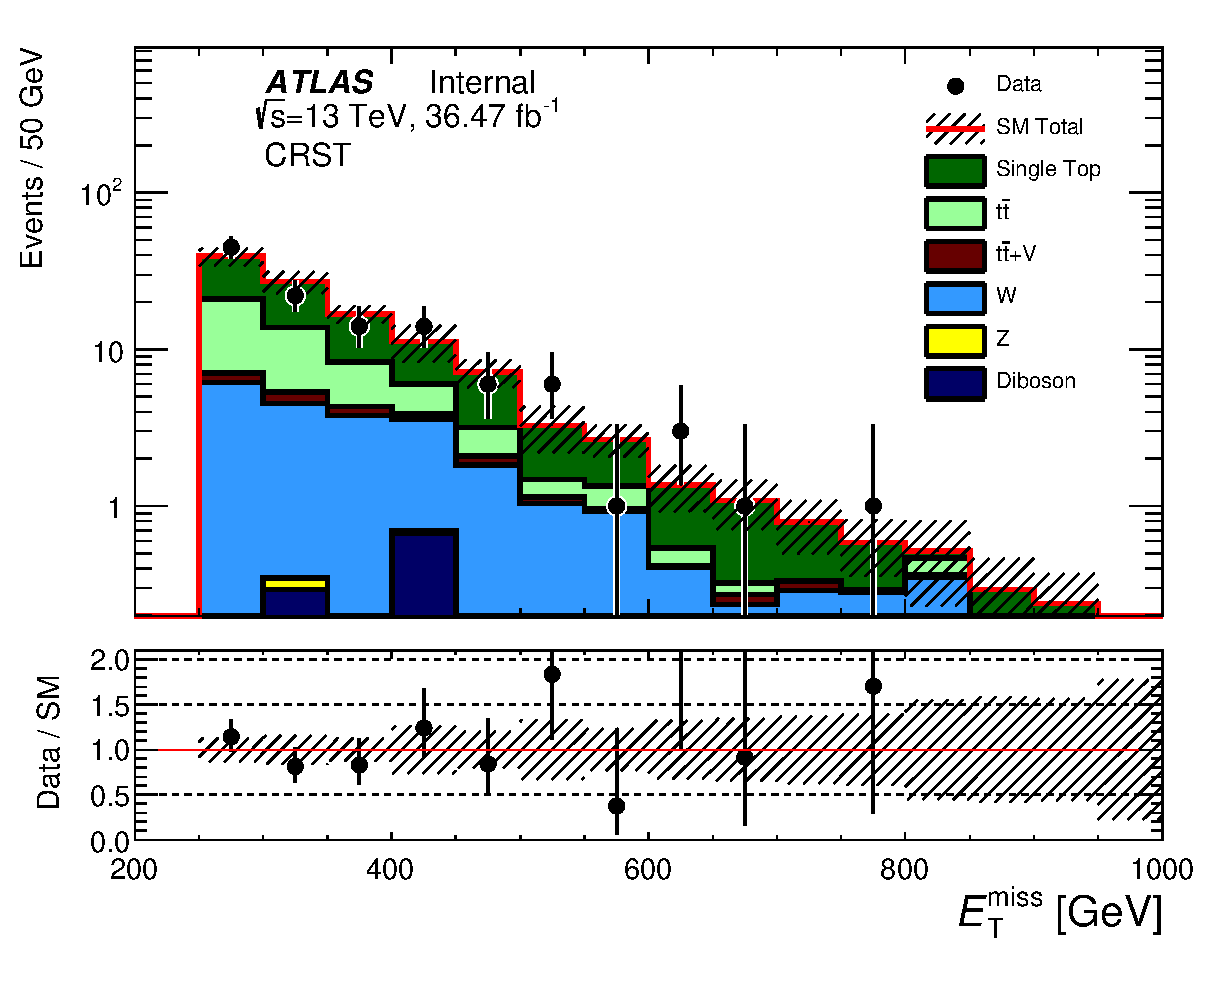
\includegraphics[width=0.45\textwidth]{figures/singleTop/postfit/Met_CRST_log.eps}
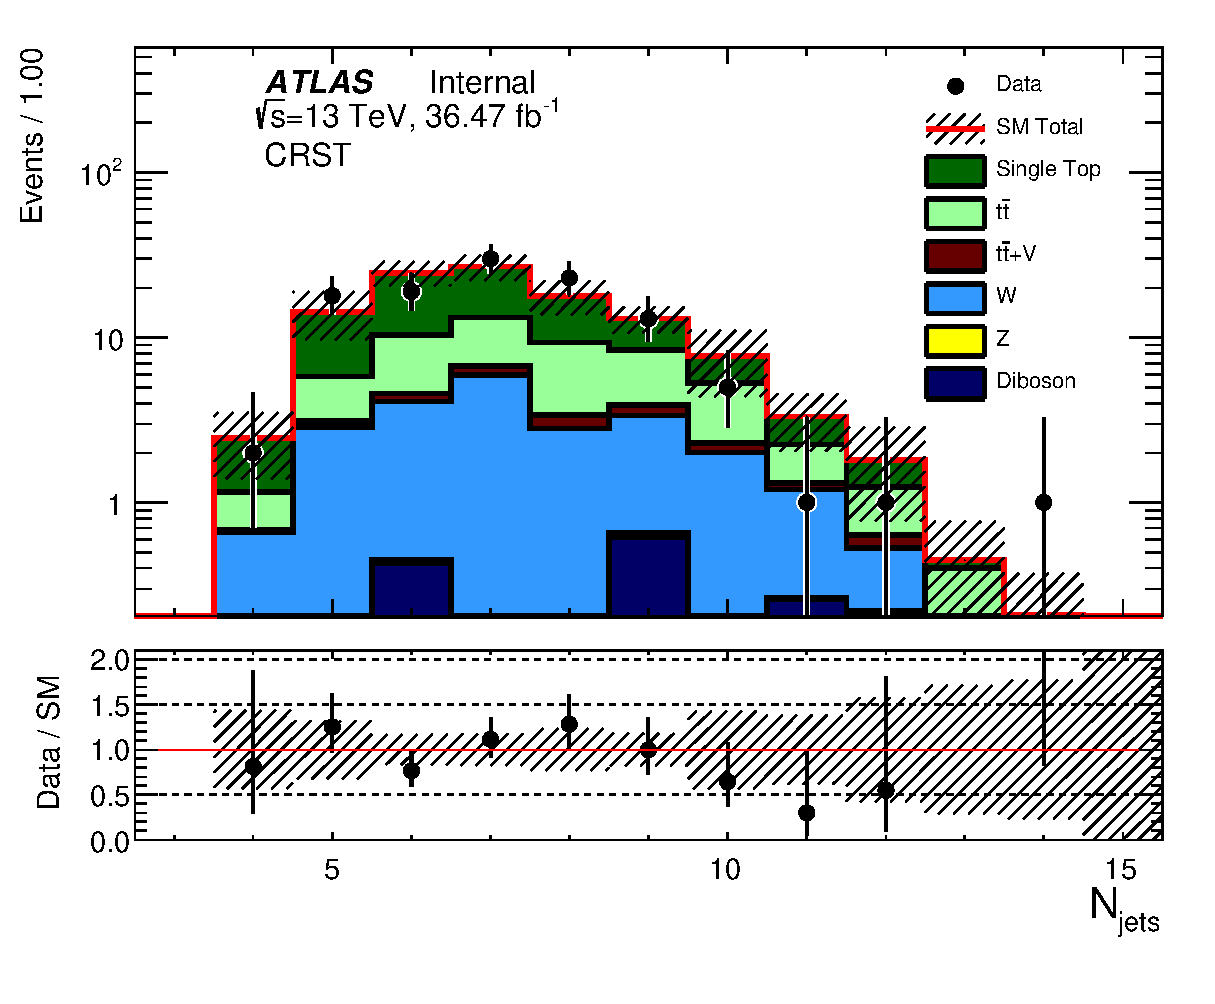
\includegraphics[width=0.45\textwidth]{figures/singleTop/postfit/NJets_CRST_log.eps}
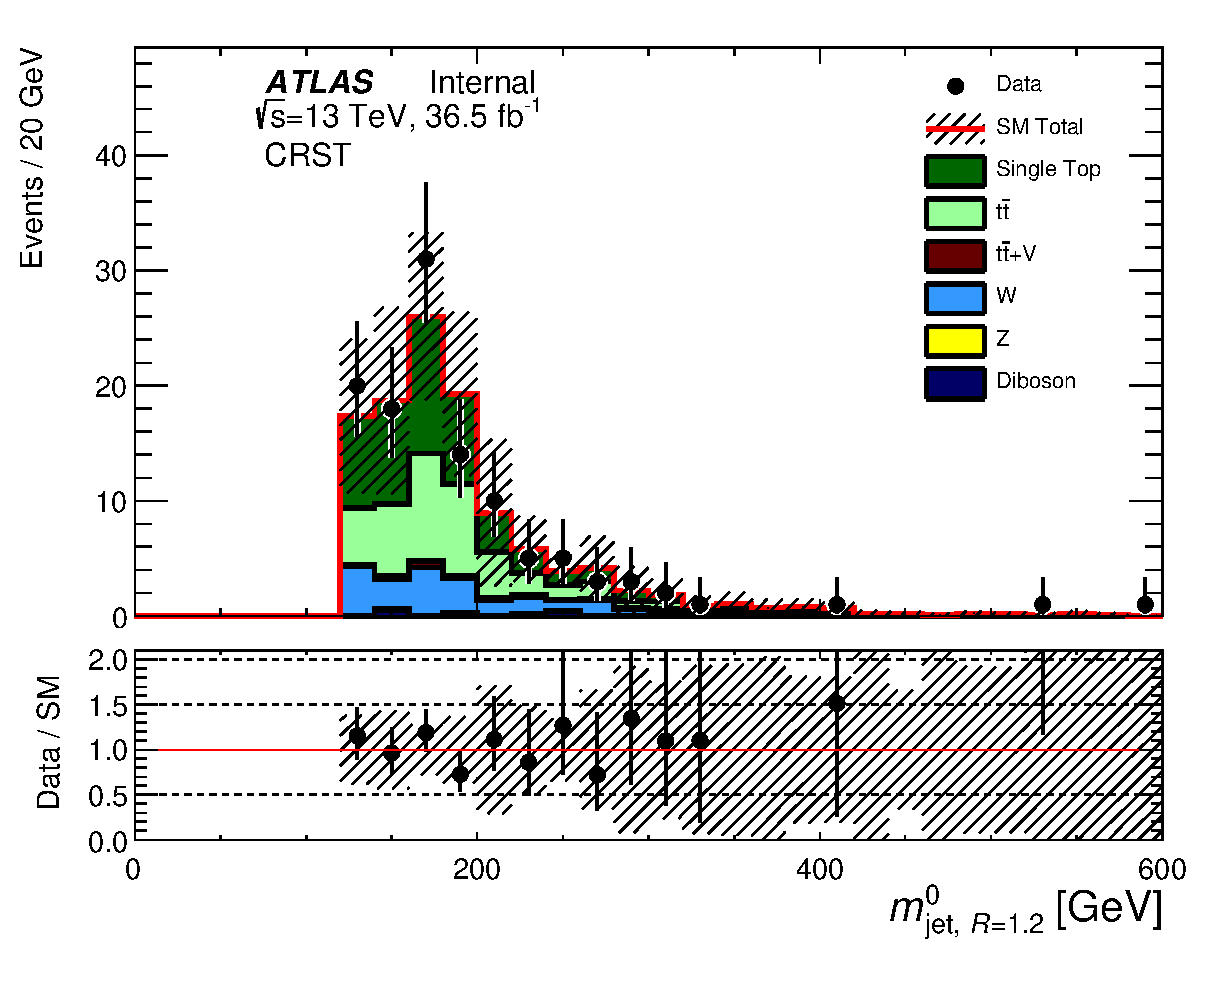
\includegraphics[width=0.45\textwidth]{figures/singleTop/postfit/AntiKt12M_0__CRST.eps}
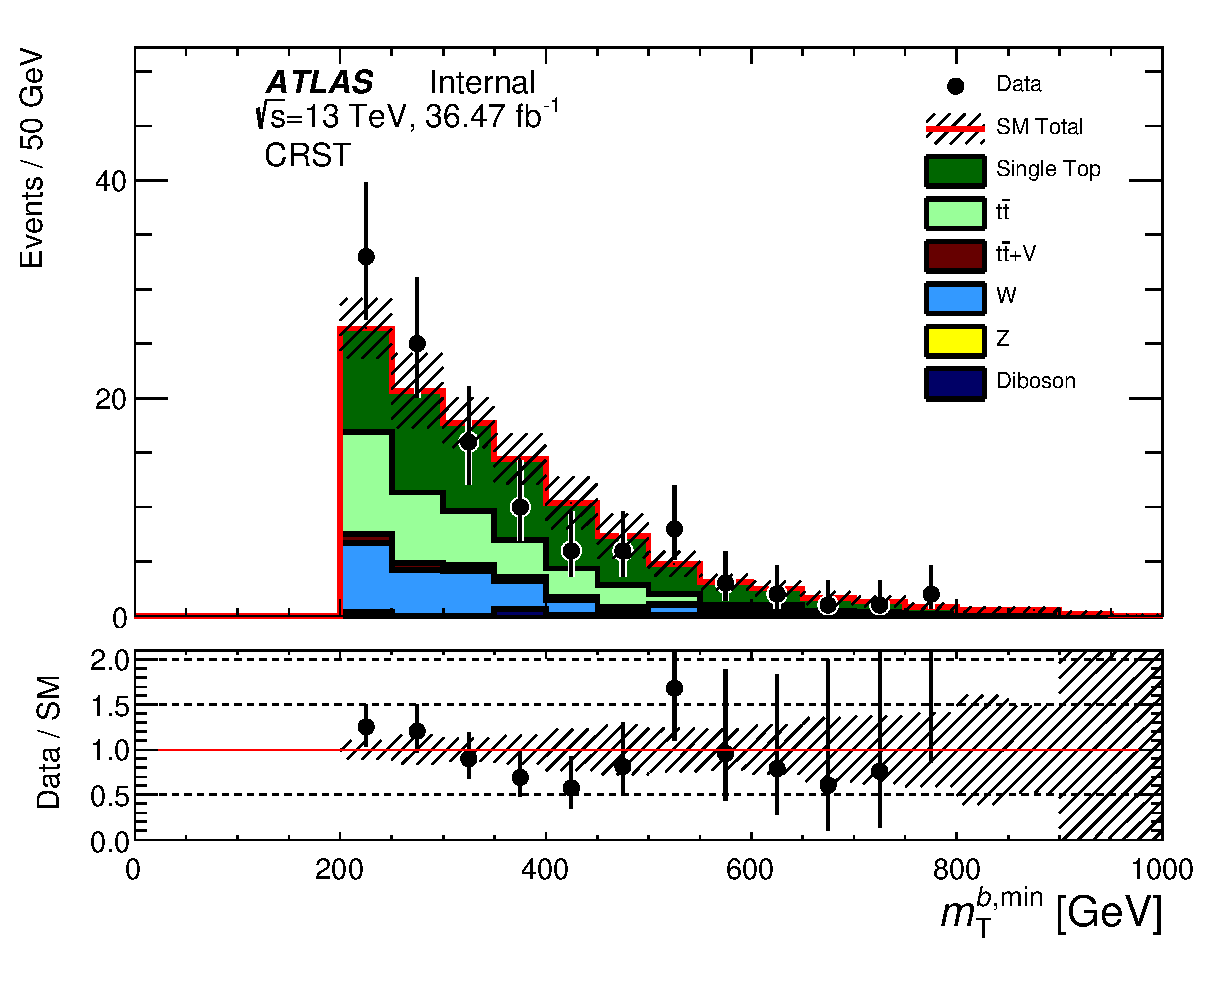
\includegraphics[width=0.45\textwidth]{figures/singleTop/postfit/MtBMin_CRST.eps}
%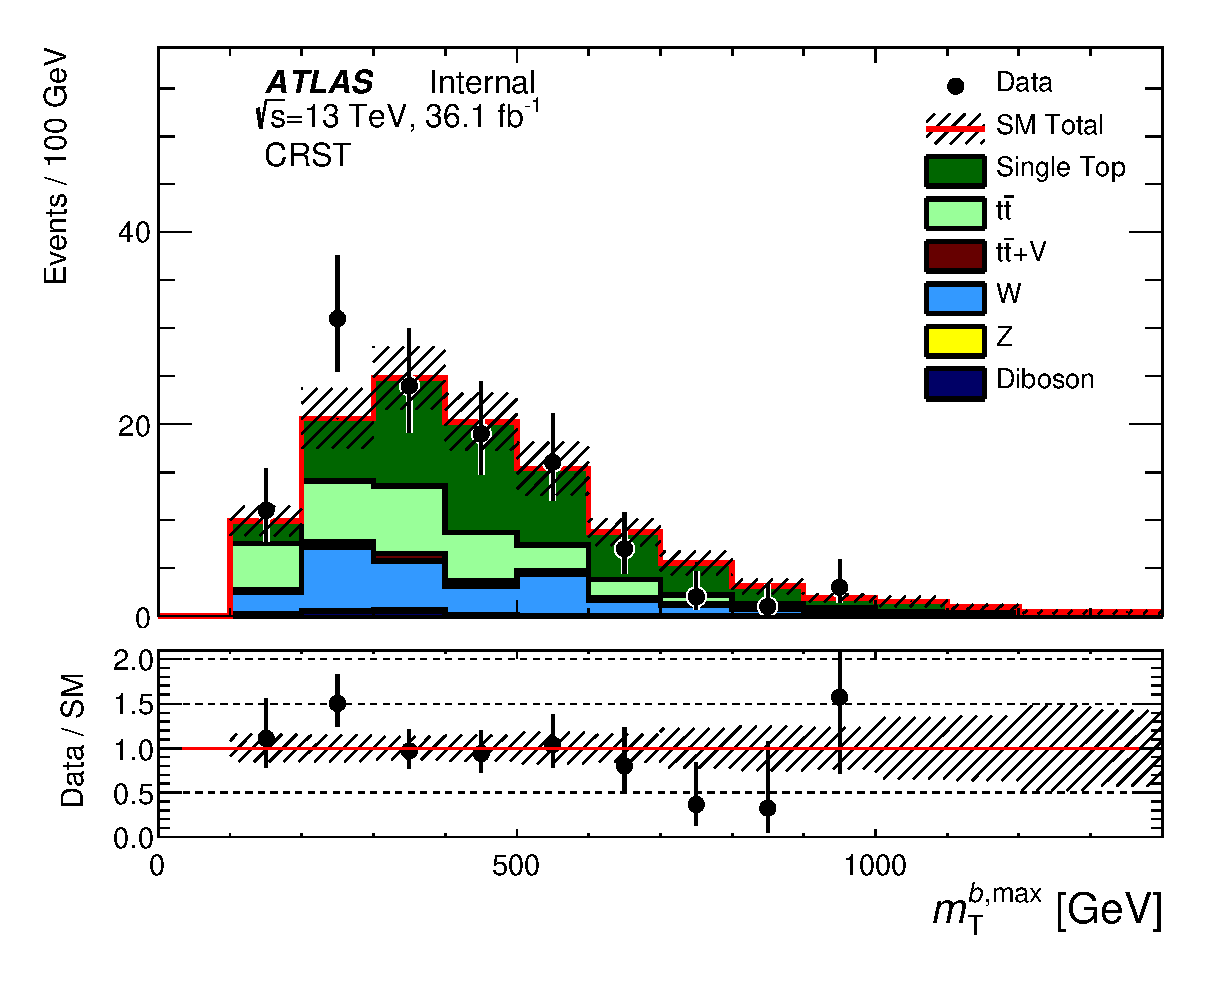
\includegraphics[width=0.45\textwidth]{figures/singleTop/postfit/MtBMax_CRST.eps}
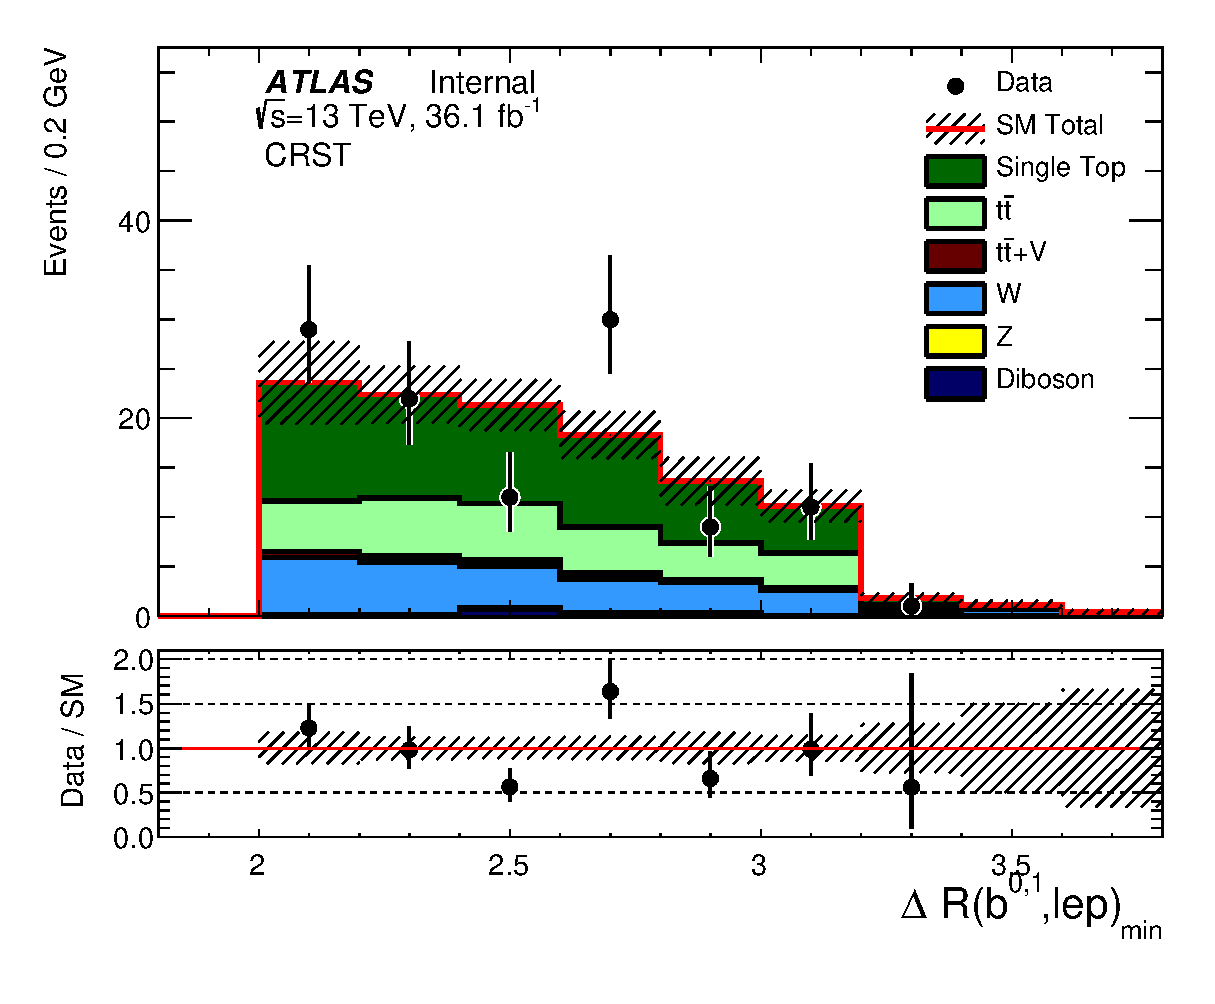
\includegraphics[width=0.45\textwidth]{figures/singleTop/postfit/MinDRBLep_CRST.eps}
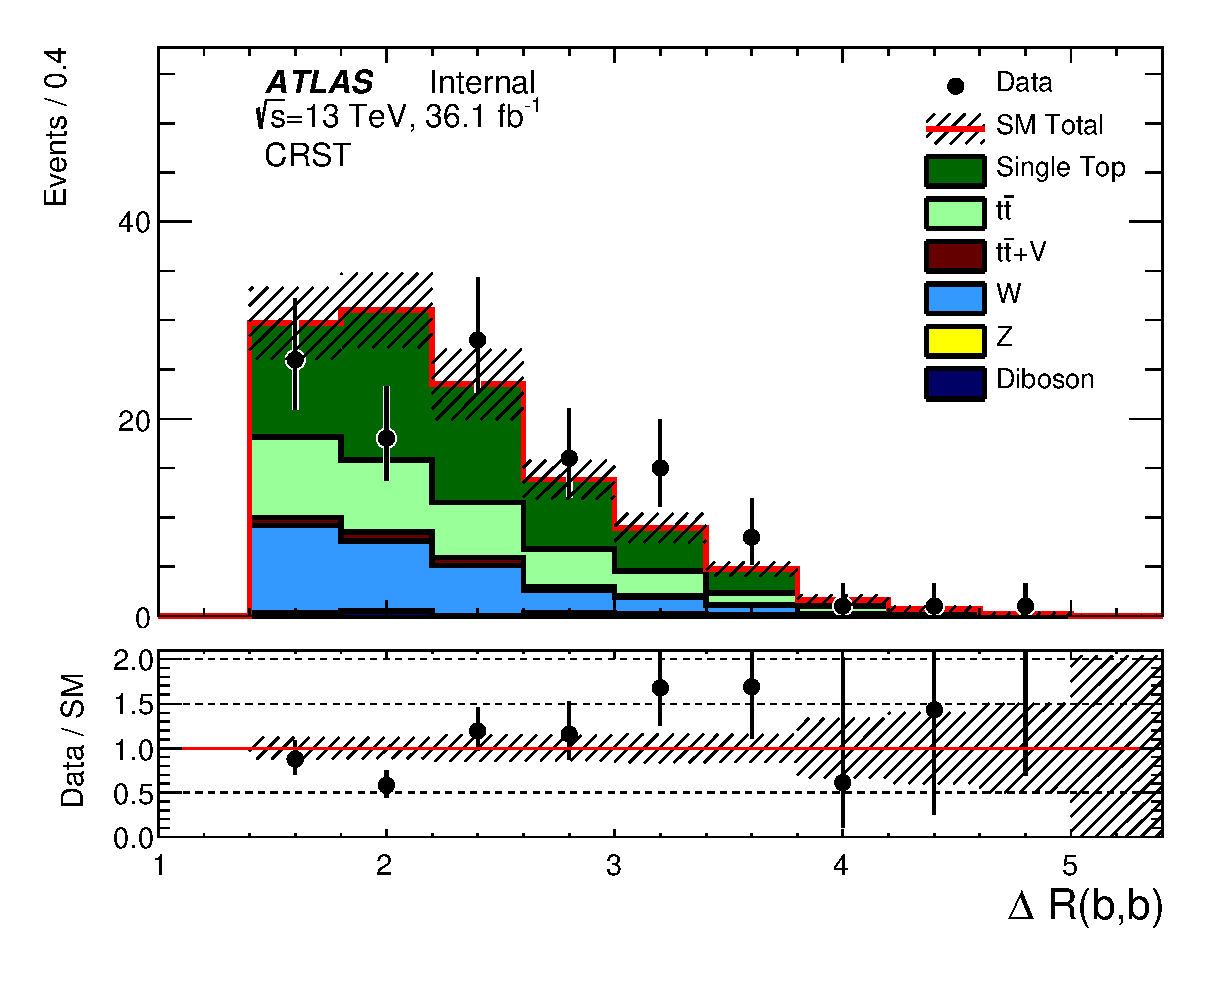
\includegraphics[width=0.45\textwidth]{figures/singleTop/postfit/DRBB_CRST.eps}
%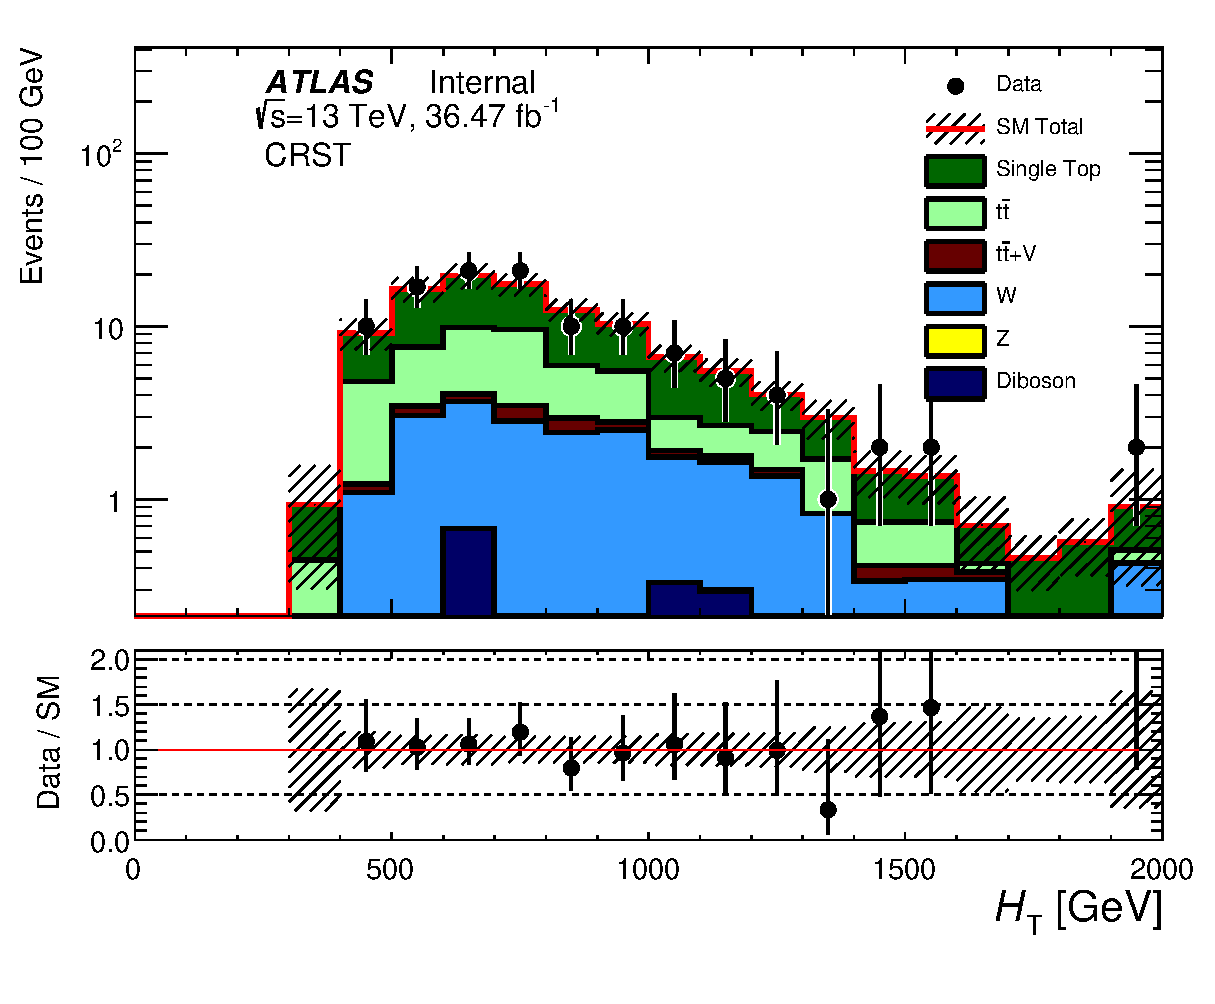
\includegraphics[width=0.45\textwidth]{figures/singleTop/postfit/Ht_CRST_log.eps}
%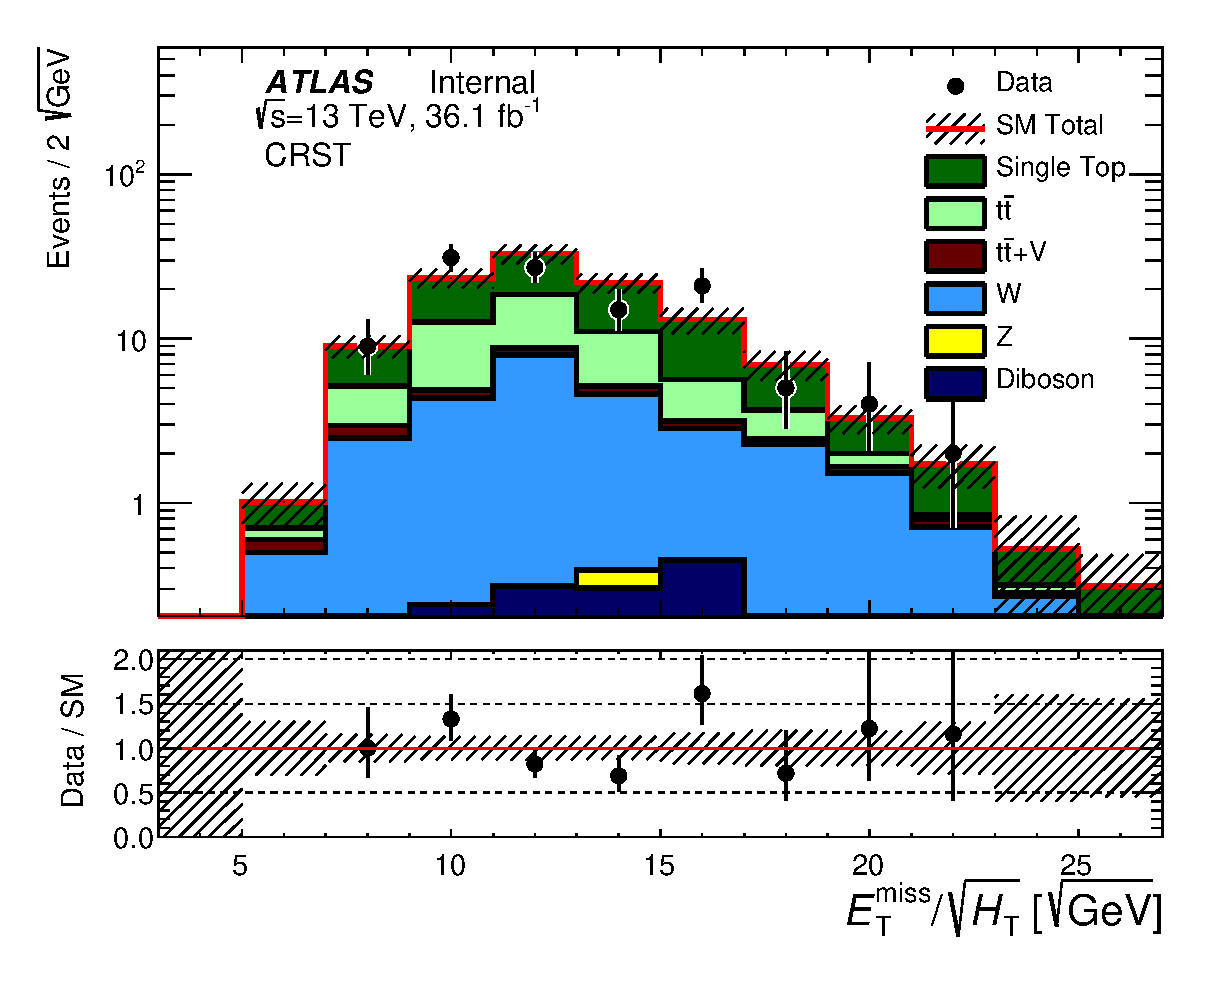
\includegraphics[width=0.45\textwidth]{figures/singleTop/postfit/HtSig_CRST_log.eps}
\end{center}
\caption{Single top control region distributions for \intlumi\ \ifb\ of data after a simultaneous fit to all background CR. The ratio between data and MC is shown in the bottom panel. The hashed area on the expected SM background represent the uncertainty due to experimental systematics and MC statistics.}
\label{fig:CRST}
\end{figure}


\clearpage